\documentclass[conference]{IEEEtran}
\IEEEoverridecommandlockouts
% The preceding line is only needed to identify funding in the first footnote. If that is unneeded, please comment it out.
\usepackage{cite}
\usepackage[portuges,brazil,english]{babel}
\usepackage{amsmath,amssymb,amsfonts}
\usepackage{algorithmic}
\usepackage{graphicx}
\usepackage{textcomp}
\def\BibTeX{{\rm B\kern-.05em{\sc i\kern-.025em b}\kern-.08em
    T\kern-.1667em\lower.7ex\hbox{E}\kern-.125emX}}
\begin{document}

\title{Report Title}

\author{
\IEEEauthorblockN{Felipe Lemes Galvão}
\IEEEauthorblockA{
  RA 116790
  email address}
\and
\IEEEauthorblockN{William Hideki Azana Tustumi}
\IEEEauthorblockA{
  RA 120281
  email address}
\and
\IEEEauthorblockN{Leo Yuuki Omori Omi}
\IEEEauthorblockA{
  RA 138684
  leoyuuki@gmail.com}
\and
\IEEEauthorblockN{João Pedro Ramos Lopes}
\IEEEauthorblockA{
  RA 139546
  email address}
}

\maketitle

\section{Introduction}

This project will focus on the problem of Web Traffic Time Series Forecasting hosted on Kaggle \cite{kaggle}.
The problem focuses on the problem of forecasting the future values of multiple time series. Sequential or temporal observations emerge in many key real-world problems, ranging from biological data, financial markets, weather forecasting, to audio and video processing. The field of time series encapsulates many different problems, ranging from analysis and inference to classification and forecast. On our project we will forecast future web traffic for approximately Wikipedia pages, with a dataset provided by Kaggle \cite{kaggle_data}.

\section{Dataset Analysis}
The first step was performing an analysis of the data to understand which patterns could leverage our learning methods. Plotting graphs of the traffic from a few pages we observesd that different pages show remarkably different trends in traffic. This suggests that a good model needs to explicitly distinguish pages.
For specific pages we note a strong year-to-year autocorrelation. We also observed weaker week-to-week and month-to-month trends. One clear example of this case was the Thanksgiving holiday page that showed an yearly spike around a Wednesday on late November, around the date of the holiday.

\begin{figure}[h!]
  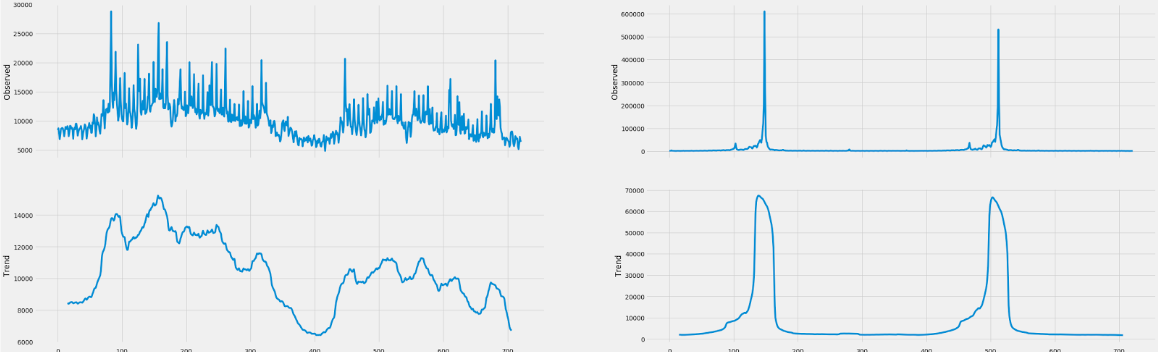
\includegraphics[width=\linewidth]{analysis1.png}
  \caption{Observed Traffic and Traffic Trend from two different pages}
  \label{fig:analysis1}
\end{figure}

Additionally, we have to deal with spikes intraffic not following a regular pattern. We note a short-term dependency following those spikes, which means the days immediately before the prediction are important to consider.

\section{Proposed Solutions}
Considering the type of data we decided to solve the problem using Long Short Term Memory networks (LSTM) as it is a natural way to model problem. As a comparison, Multilayer perceptron was also implemented (MLP). From our analysis of the data, the input of our networks is the day of the year, page id and page views from the previous day or week.

\subsection{Long Short Term Memory networks}

Our implementation of the LSTM applies Backpropagation Through Time (BPTT) after each time step and uses batch normalization to avoid exploding gradients.
The model combines previous occurrences with data extracted from the current steps. So it receives page unique id, day from the start of the series and number of visits of the last day as input.

\begin{figure}[h!]
  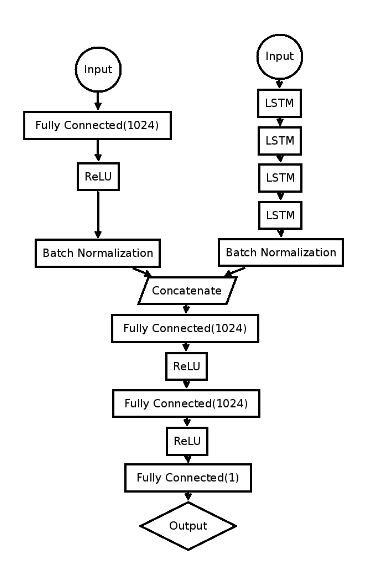
\includegraphics[width=\linewidth]{lstm.png}
  \caption{Observed Traffic and Traffic Trend from two different pages}
  \label{fig:analysis1}
\end{figure}

\section{Experiments and Discussion}

The experiments carried out and the obtained
results.

\section{Conclusions and Future Work}

The main conclusions of the work as well as some future directions for other people interested in continuing this work. 

\begin{thebibliography}{00}
\bibitem{kaggle}
  Kaggle,
  \textit{Web Traffic Time Series Forecasting},
  https://www.kaggle.com/c/web-traffic-time-series-forecasting
\bibitem{kaggle_data}
  Kaggle,
  \textit{Web Traffic Time Series Forecasting Data},
  https://www.kaggle.com/c/web-traffic-time-series-forecasting/data
\end{thebibliography}

\end{document}
